\section{VTrack Class Reference}
\label{classVTrack}\index{VTrack@{VTrack}}
{\tt \#include $<$vtrack.h$>$}

Collaboration diagram for VTrack:\begin{figure}[H]
\begin{center}
\leavevmode
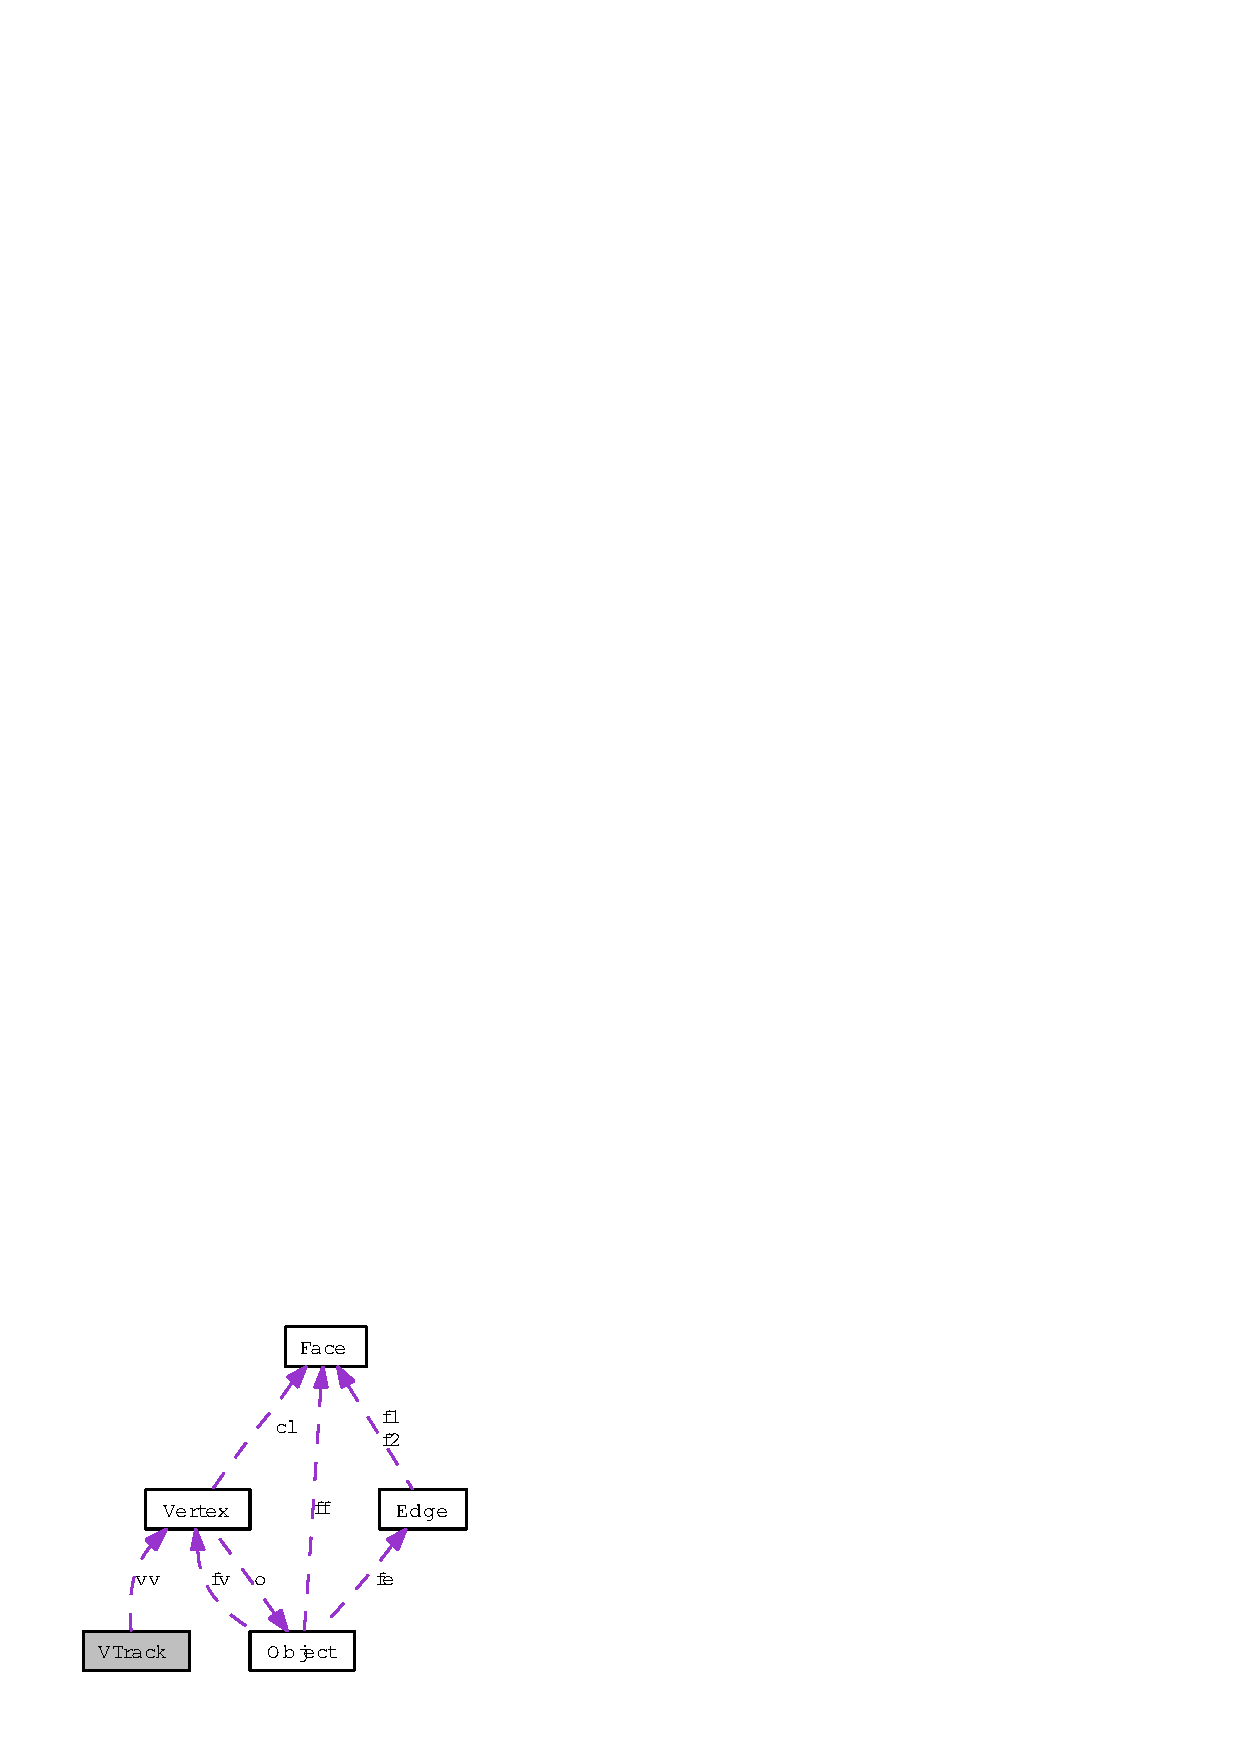
\includegraphics[width=114pt]{classVTrack__coll__graph}
\end{center}
\end{figure}
\subsection*{Public Member Functions}
\begin{CompactItemize}
\item 
{\bf VTrack} (void)
\item 
{\bf VTrack} ({\bf VTrack} const \&)
\item 
{\bf VTrack} \& {\bf operator=} ({\bf VTrack} const \&)
\item 
bool {\bf is\-Good} (void)
\item 
void {\bf clear} (void)
\item 
void {\bf print} (void)
\item 
void {\bf print\-Bad} (void)
\item 
void {\bf add\-New\-Sep\-Dis} (double)
\item 
void {\bf add\-Orig\-P} ({\bf vec\_\-d} const $\ast$const)
\item 
void {\bf add\-New\-P} ({\bf vec\_\-d} const $\ast$const)
\item 
void {\bf add\-Orig\-CP} (double[3])
\item 
void {\bf add\-New\-CP} (double[3])
\item 
void {\bf add\-Vertex} ({\bf Vertex} $\ast$)
\item 
void {\bf add\-New\-VD} (double)
\item 
void {\bf add\-New\-Top\-N} (double)
\item 
void {\bf add\-Orig\-Sep\-Dis} (double)
\item 
void {\bf add\-Orig\-VD} (double)
\item 
void {\bf add\-Orig\-Top\-N} (double)
\item 
void {\bf premove} ({\bf Vertex} $\ast$)
\item 
void {\bf postmove} (void)
\item 
double {\bf get\-New\-Sep\-Dis} (void)
\item 
double {\bf get\-New\-VD} (void)
\item 
double {\bf get\-New\-Top\-N} (void)
\item 
double {\bf get\-Orig\-Sep\-Dis} (void)
\item 
double {\bf get\-Orig\-VD} (void)
\item 
double {\bf get\-Orig\-Top\-N} (void)
\item 
{\bf Vertex} $\ast$ {\bf get\-Vertex} (void)
\end{CompactItemize}


\subsection{Detailed Description}




Definition at line 6 of file vtrack.h.

\subsection{Constructor \& Destructor Documentation}
\index{VTrack@{VTrack}!VTrack@{VTrack}}
\index{VTrack@{VTrack}!VTrack@{VTrack}}
\subsubsection{\setlength{\rightskip}{0pt plus 5cm}VTrack::VTrack (void)}\label{classVTrack_70105fe97cc4d64bf6c594145b889083}




Definition at line 14 of file vtrack.cc.\index{VTrack@{VTrack}!VTrack@{VTrack}}
\index{VTrack@{VTrack}!VTrack@{VTrack}}
\subsubsection{\setlength{\rightskip}{0pt plus 5cm}VTrack::VTrack ({\bf VTrack} const \&)}\label{classVTrack_9ccc41f55cda6014ad427c6aecab37d7}




Definition at line 21 of file vtrack.cc.

References Vertex::get\-Index(), and vv.

Here is the call graph for this function:\begin{figure}[H]
\begin{center}
\leavevmode
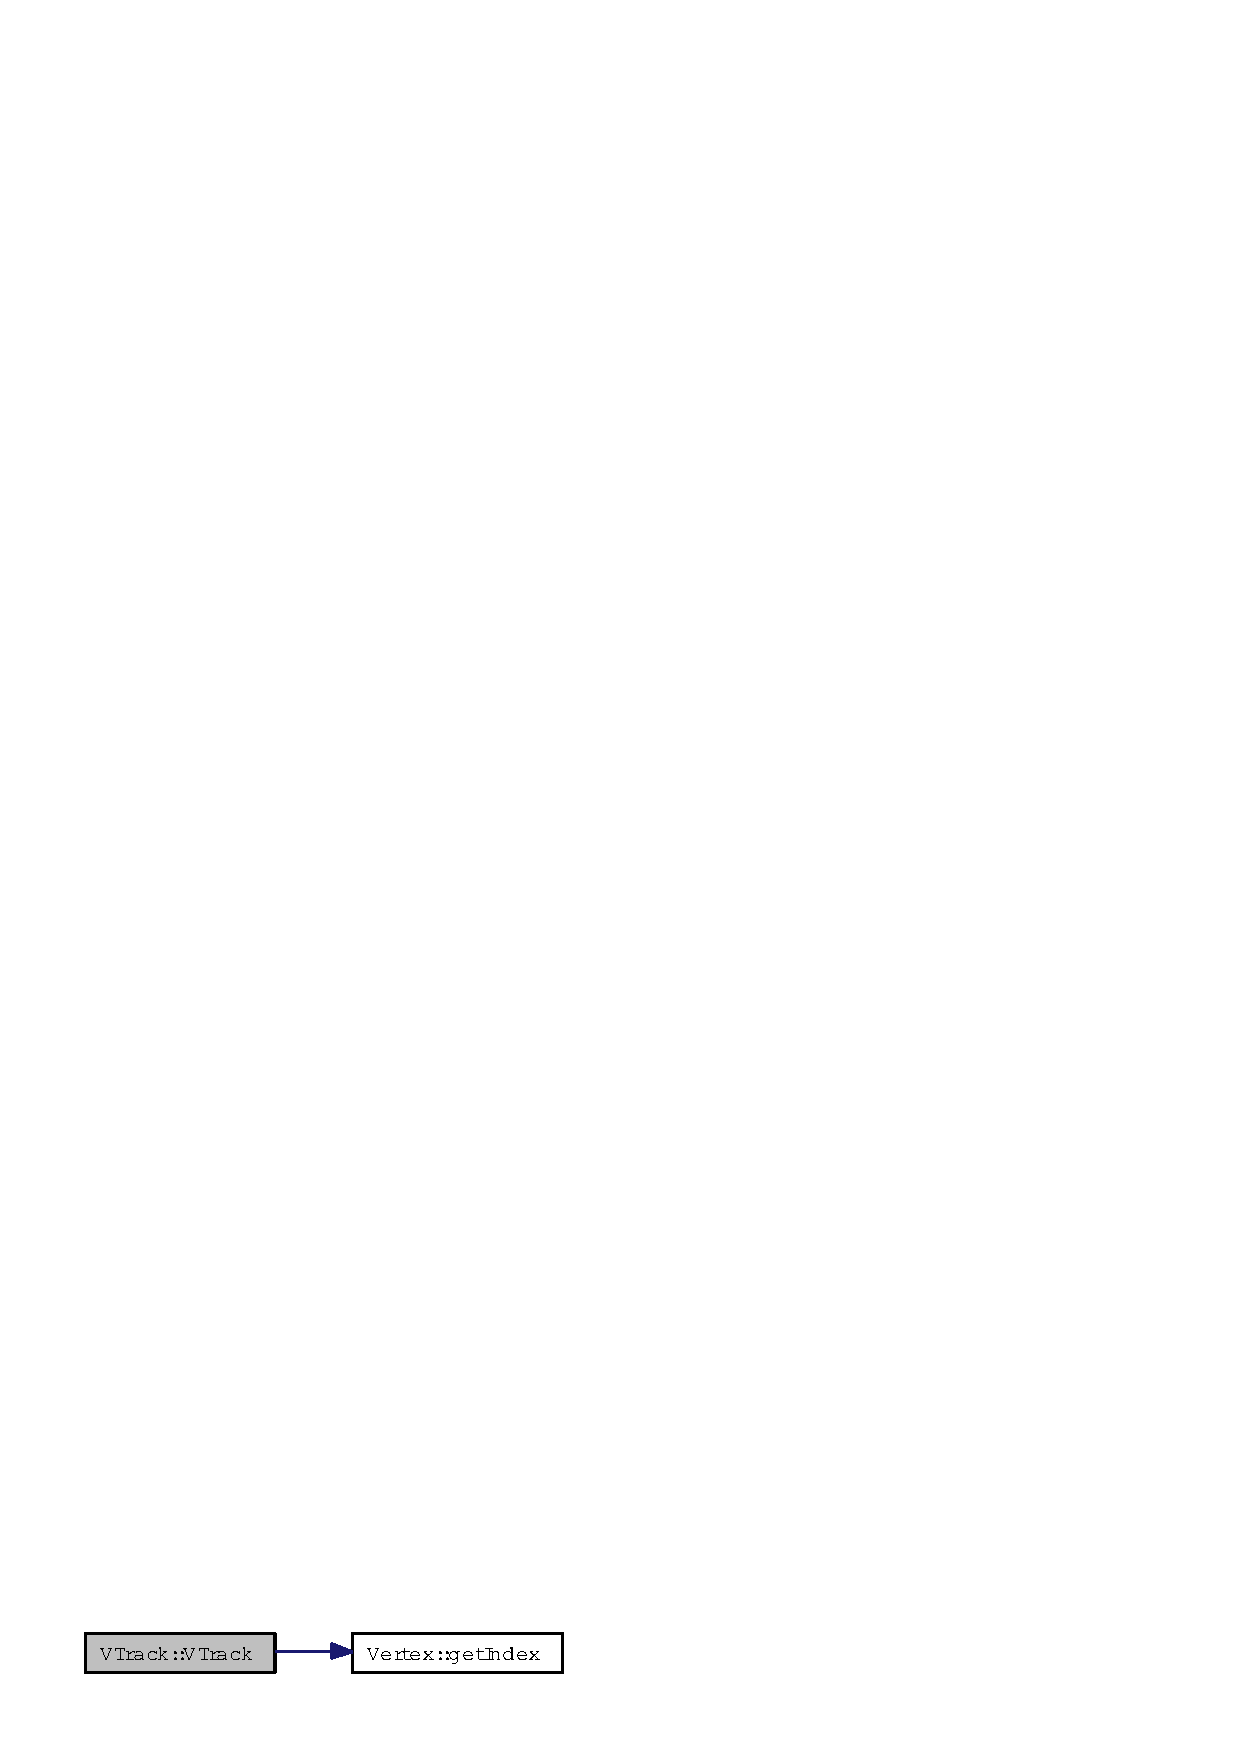
\includegraphics[width=137pt]{classVTrack_9ccc41f55cda6014ad427c6aecab37d7_cgraph}
\end{center}
\end{figure}


\subsection{Member Function Documentation}
\index{VTrack@{VTrack}!operator=@{operator=}}
\index{operator=@{operator=}!VTrack@{VTrack}}
\subsubsection{\setlength{\rightskip}{0pt plus 5cm}{\bf VTrack} \& VTrack::operator= ({\bf VTrack} const \&)}\label{classVTrack_9b0cc4eb615943338033f9d07fd52e48}




Definition at line 31 of file vtrack.cc.

References Vertex::get\-Index(), and vv.

Here is the call graph for this function:\begin{figure}[H]
\begin{center}
\leavevmode
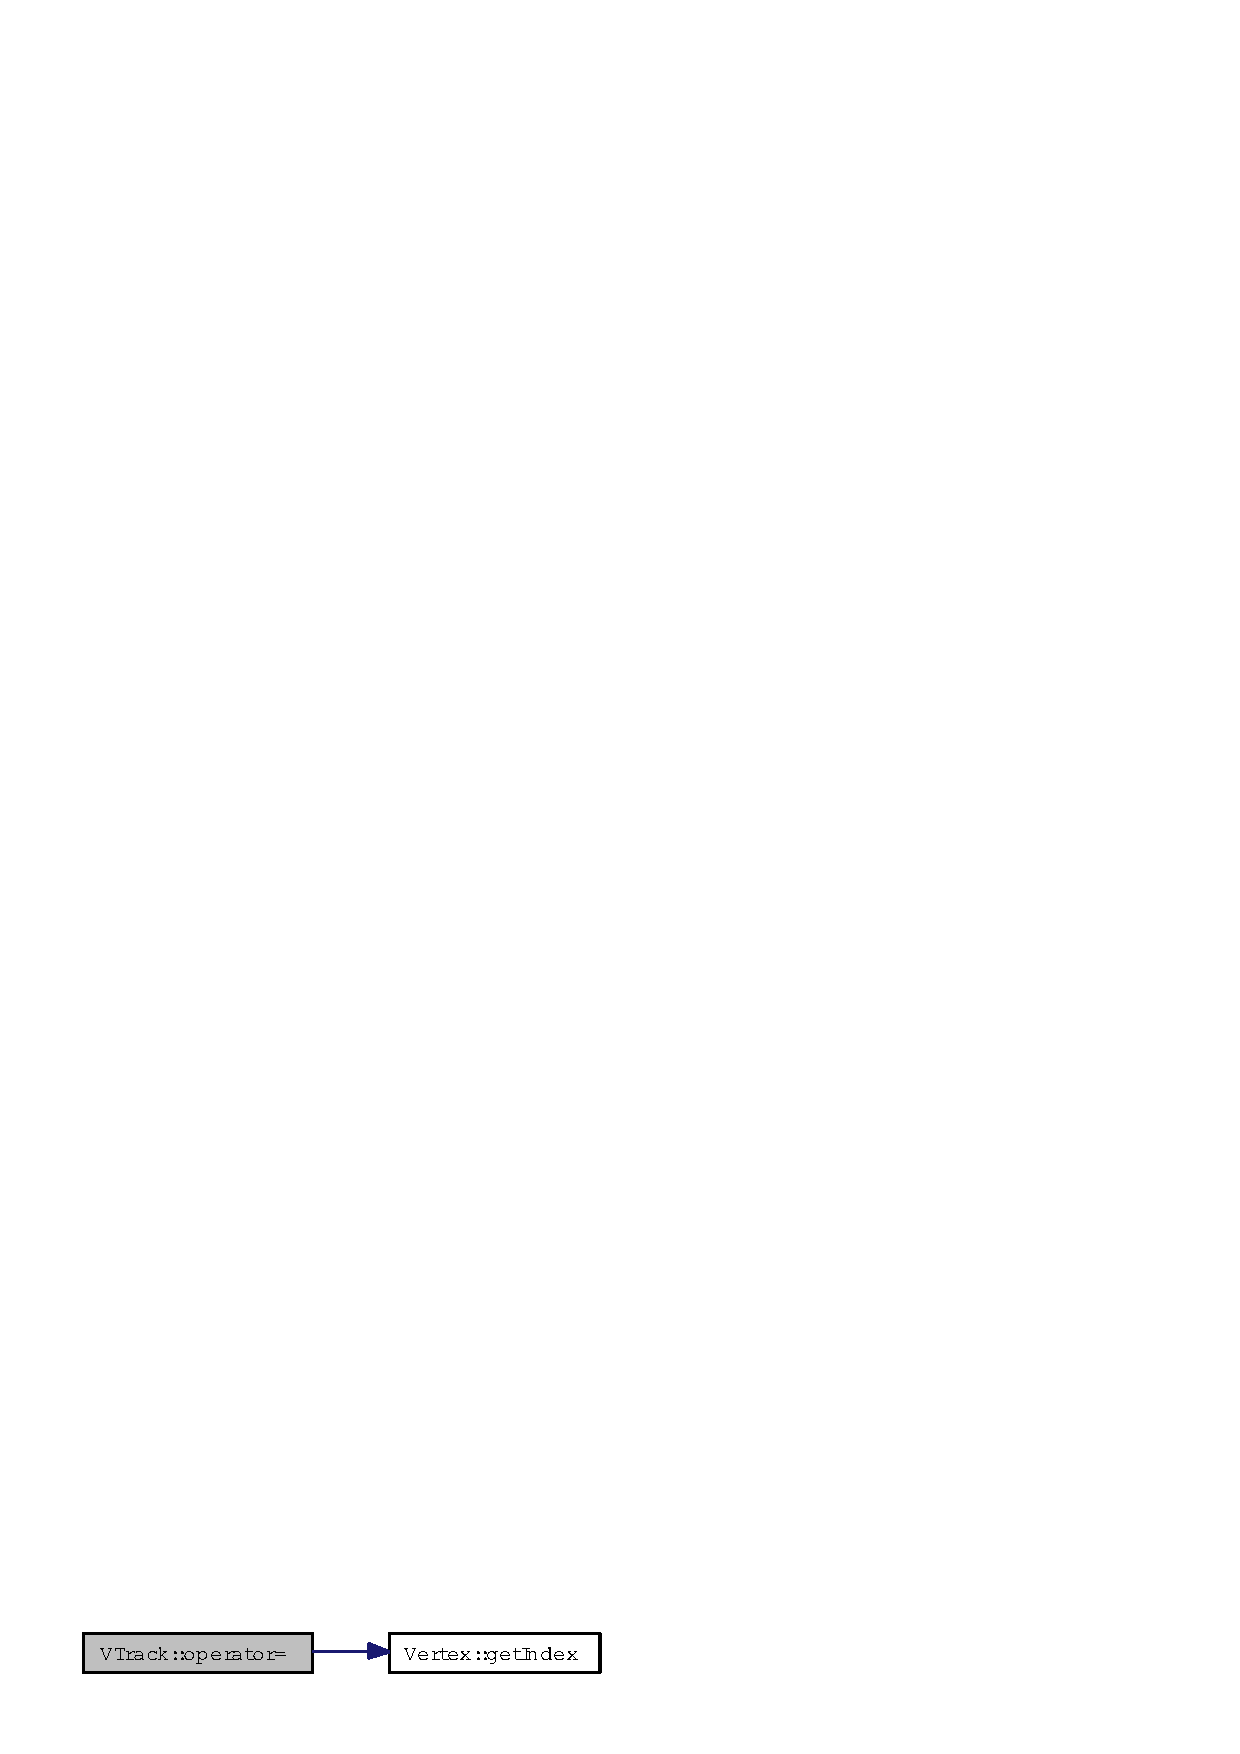
\includegraphics[width=146pt]{classVTrack_9b0cc4eb615943338033f9d07fd52e48_cgraph}
\end{center}
\end{figure}
\index{VTrack@{VTrack}!isGood@{isGood}}
\index{isGood@{isGood}!VTrack@{VTrack}}
\subsubsection{\setlength{\rightskip}{0pt plus 5cm}bool VTrack::is\-Good (void)}\label{classVTrack_ca6c7a71f823e2e65861a6a0b77953d5}




Definition at line 100 of file vtrack.cc.

Referenced by postmove().\index{VTrack@{VTrack}!clear@{clear}}
\index{clear@{clear}!VTrack@{VTrack}}
\subsubsection{\setlength{\rightskip}{0pt plus 5cm}void VTrack::clear (void)}\label{classVTrack_d1d0f87e5c865a9a61648ff184338460}




Definition at line 175 of file vtrack.cc.

Referenced by premove().\index{VTrack@{VTrack}!print@{print}}
\index{print@{print}!VTrack@{VTrack}}
\subsubsection{\setlength{\rightskip}{0pt plus 5cm}void VTrack::print (void)}\label{classVTrack_17a4d3fb66d3641a39b519cfe9a51986}




Definition at line 63 of file vtrack.cc.

Referenced by postmove().\index{VTrack@{VTrack}!printBad@{printBad}}
\index{printBad@{printBad}!VTrack@{VTrack}}
\subsubsection{\setlength{\rightskip}{0pt plus 5cm}void VTrack::print\-Bad (void)}\label{classVTrack_d17ae565fa54b47aabf0ba8122f7cac8}




Definition at line 38 of file vtrack.cc.

Referenced by postmove().\index{VTrack@{VTrack}!addNewSepDis@{addNewSepDis}}
\index{addNewSepDis@{addNewSepDis}!VTrack@{VTrack}}
\subsubsection{\setlength{\rightskip}{0pt plus 5cm}void VTrack::add\-New\-Sep\-Dis (double)}\label{classVTrack_67a17c76271d4ae43736ca23e6d06a67}




Definition at line 115 of file vtrack.cc.

Referenced by postmove().\index{VTrack@{VTrack}!addOrigP@{addOrigP}}
\index{addOrigP@{addOrigP}!VTrack@{VTrack}}
\subsubsection{\setlength{\rightskip}{0pt plus 5cm}void VTrack::add\-Orig\-P ({\bf vec\_\-d} const $\ast$ {\em const})}\label{classVTrack_aa3b7b2b501c7d23a3509c89ae617c26}




Definition at line 194 of file vtrack.cc.

Referenced by premove().\index{VTrack@{VTrack}!addNewP@{addNewP}}
\index{addNewP@{addNewP}!VTrack@{VTrack}}
\subsubsection{\setlength{\rightskip}{0pt plus 5cm}void VTrack::add\-New\-P ({\bf vec\_\-d} const $\ast$ {\em const})}\label{classVTrack_45a34666d8cd52ec28164f8c1bc5f754}




Definition at line 222 of file vtrack.cc.

Referenced by postmove().\index{VTrack@{VTrack}!addOrigCP@{addOrigCP}}
\index{addOrigCP@{addOrigCP}!VTrack@{VTrack}}
\subsubsection{\setlength{\rightskip}{0pt plus 5cm}void VTrack::add\-Orig\-CP (double[3])}\label{classVTrack_f13f7d2b9207e392ed9c17f1ed617aed}




Definition at line 229 of file vtrack.cc.

Referenced by premove().\index{VTrack@{VTrack}!addNewCP@{addNewCP}}
\index{addNewCP@{addNewCP}!VTrack@{VTrack}}
\subsubsection{\setlength{\rightskip}{0pt plus 5cm}void VTrack::add\-New\-CP (double[3])}\label{classVTrack_f94c5aa8a9c0fdaef8e8307f52467488}




Definition at line 250 of file vtrack.cc.

Referenced by postmove().\index{VTrack@{VTrack}!addVertex@{addVertex}}
\index{addVertex@{addVertex}!VTrack@{VTrack}}
\subsubsection{\setlength{\rightskip}{0pt plus 5cm}void VTrack::add\-Vertex ({\bf Vertex} $\ast$)}\label{classVTrack_92f6a3668ad24dce5ae5fa49c39b9196}




Definition at line 95 of file vtrack.cc.

Referenced by premove().\index{VTrack@{VTrack}!addNewVD@{addNewVD}}
\index{addNewVD@{addNewVD}!VTrack@{VTrack}}
\subsubsection{\setlength{\rightskip}{0pt plus 5cm}void VTrack::add\-New\-VD (double)}\label{classVTrack_149d5c6161c842d3f3e36df7e4cc8efc}




Definition at line 125 of file vtrack.cc.

Referenced by postmove().\index{VTrack@{VTrack}!addNewTopN@{addNewTopN}}
\index{addNewTopN@{addNewTopN}!VTrack@{VTrack}}
\subsubsection{\setlength{\rightskip}{0pt plus 5cm}void VTrack::add\-New\-Top\-N (double)}\label{classVTrack_af74c77dff5cdd41febb3cb1f4b3e383}




Definition at line 135 of file vtrack.cc.

Referenced by postmove().\index{VTrack@{VTrack}!addOrigSepDis@{addOrigSepDis}}
\index{addOrigSepDis@{addOrigSepDis}!VTrack@{VTrack}}
\subsubsection{\setlength{\rightskip}{0pt plus 5cm}void VTrack::add\-Orig\-Sep\-Dis (double)}\label{classVTrack_c2bb39280976c84ea65cb890bc41ed69}




Definition at line 145 of file vtrack.cc.

Referenced by premove().\index{VTrack@{VTrack}!addOrigVD@{addOrigVD}}
\index{addOrigVD@{addOrigVD}!VTrack@{VTrack}}
\subsubsection{\setlength{\rightskip}{0pt plus 5cm}void VTrack::add\-Orig\-VD (double)}\label{classVTrack_8ffc5476e3a6afe96e55746f07055f7c}




Definition at line 155 of file vtrack.cc.

Referenced by premove().\index{VTrack@{VTrack}!addOrigTopN@{addOrigTopN}}
\index{addOrigTopN@{addOrigTopN}!VTrack@{VTrack}}
\subsubsection{\setlength{\rightskip}{0pt plus 5cm}void VTrack::add\-Orig\-Top\-N (double)}\label{classVTrack_23f52fb1e7855437ecab15ea7b1dbf4d}




Definition at line 165 of file vtrack.cc.

Referenced by premove().\index{VTrack@{VTrack}!premove@{premove}}
\index{premove@{premove}!VTrack@{VTrack}}
\subsubsection{\setlength{\rightskip}{0pt plus 5cm}void VTrack::premove ({\bf Vertex} $\ast$)}\label{classVTrack_517d3992d6ab6751876f2697e3ade430}




Definition at line 257 of file vtrack.cc.

References add\-Orig\-CP(), add\-Orig\-P(), add\-Orig\-Sep\-Dis(), add\-Orig\-Top\-N(), add\-Orig\-VD(), add\-Vertex(), clear(), Virtual\_\-Disp::find\-Top\-N(), Container::get\-Near\-Pt\-On\-Face\-To\-Vertex(), Vertex::get\-Sq\-Sep\-Dist(), Container::instance(), Virtual\_\-Disp::instance(), and Vertex\_\-Schedule::instance().

Referenced by main().

Here is the call graph for this function:\begin{figure}[H]
\begin{center}
\leavevmode
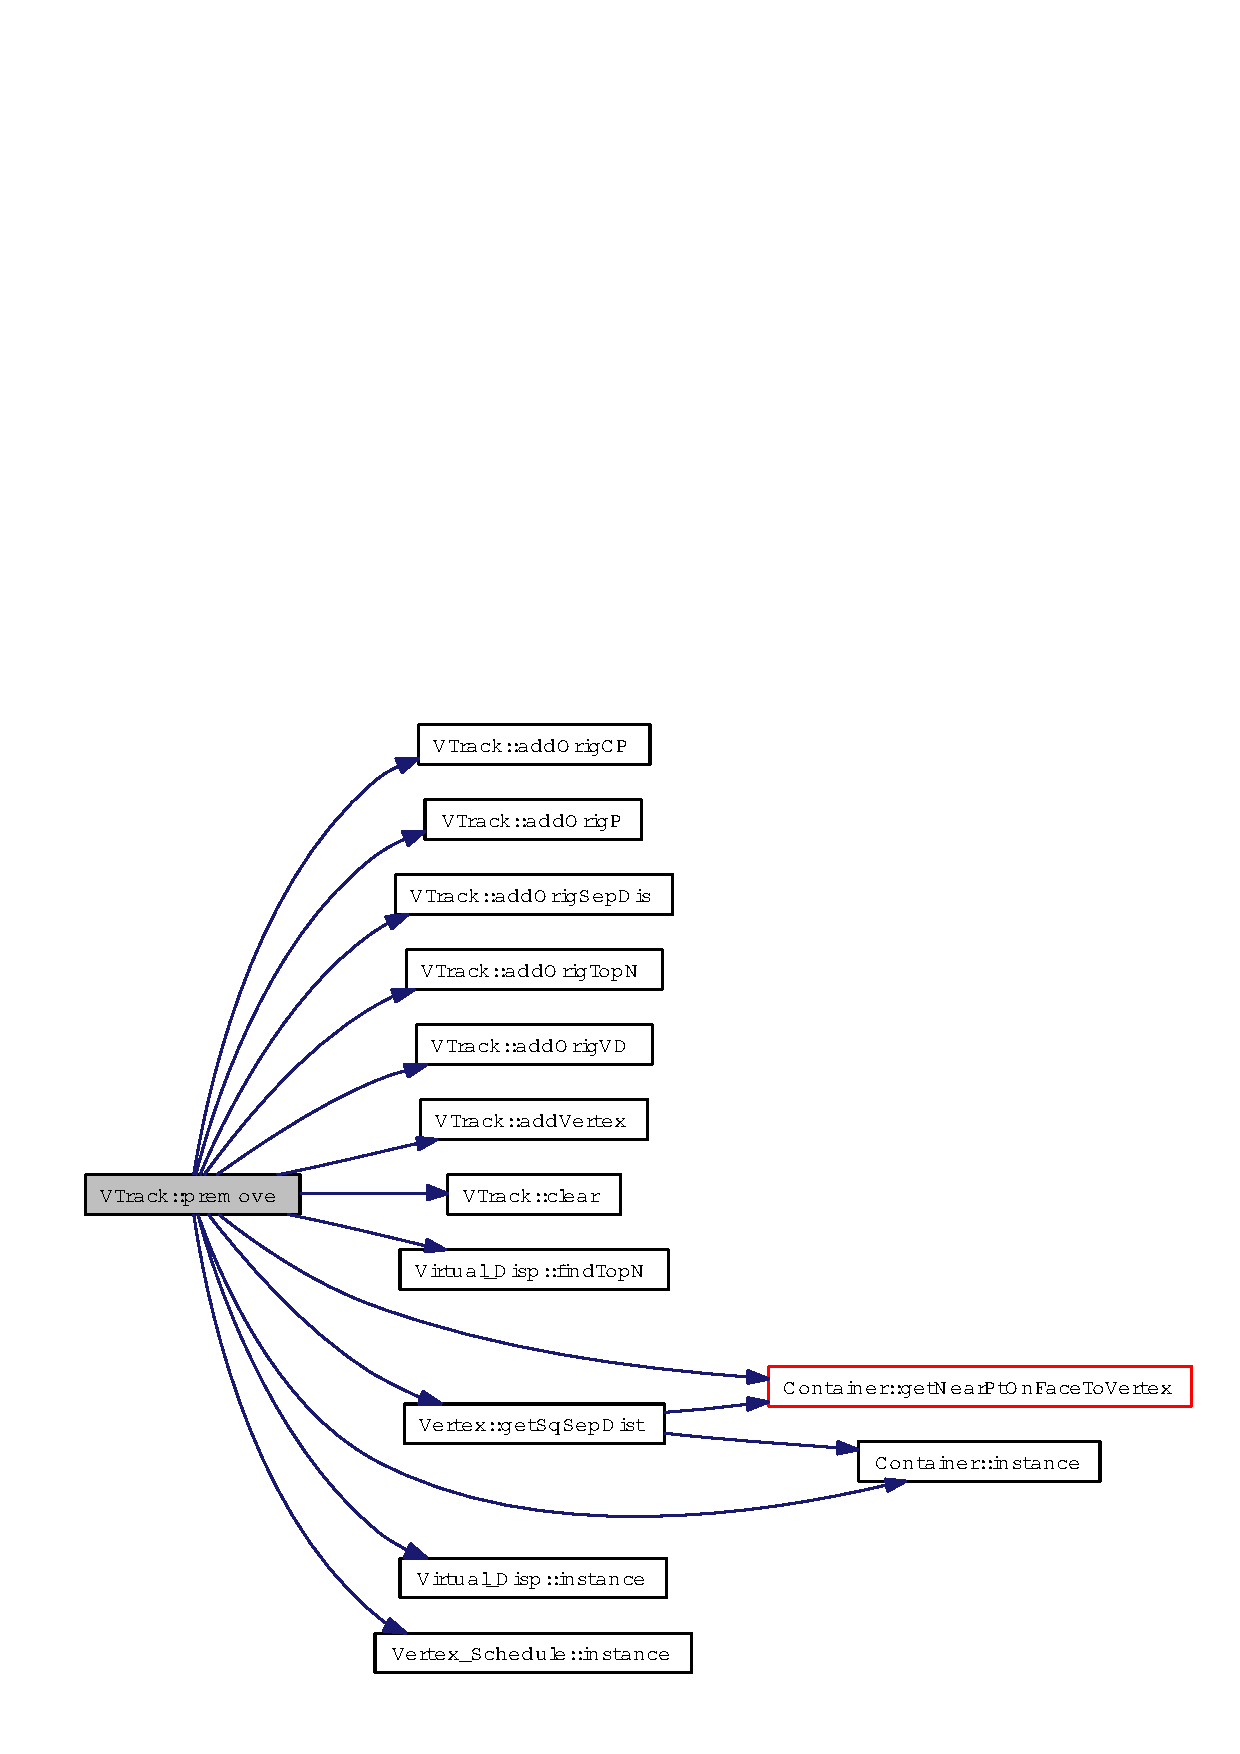
\includegraphics[width=288pt]{classVTrack_517d3992d6ab6751876f2697e3ade430_cgraph}
\end{center}
\end{figure}
\index{VTrack@{VTrack}!postmove@{postmove}}
\index{postmove@{postmove}!VTrack@{VTrack}}
\subsubsection{\setlength{\rightskip}{0pt plus 5cm}void VTrack::postmove (void)}\label{classVTrack_6cc3f121ae5886b77b7b40dee5ffe05d}




Definition at line 276 of file vtrack.cc.

References add\-New\-CP(), add\-New\-P(), add\-New\-Sep\-Dis(), add\-New\-Top\-N(), add\-New\-VD(), Virtual\_\-Disp::find\-Top\-N(), Container::get\-Near\-Pt\-On\-Face\-To\-Vertex(), Container::instance(), Virtual\_\-Disp::instance(), Vertex\_\-Schedule::instance(), is\-Good(), print(), and print\-Bad().

Referenced by main().

Here is the call graph for this function:\begin{figure}[H]
\begin{center}
\leavevmode
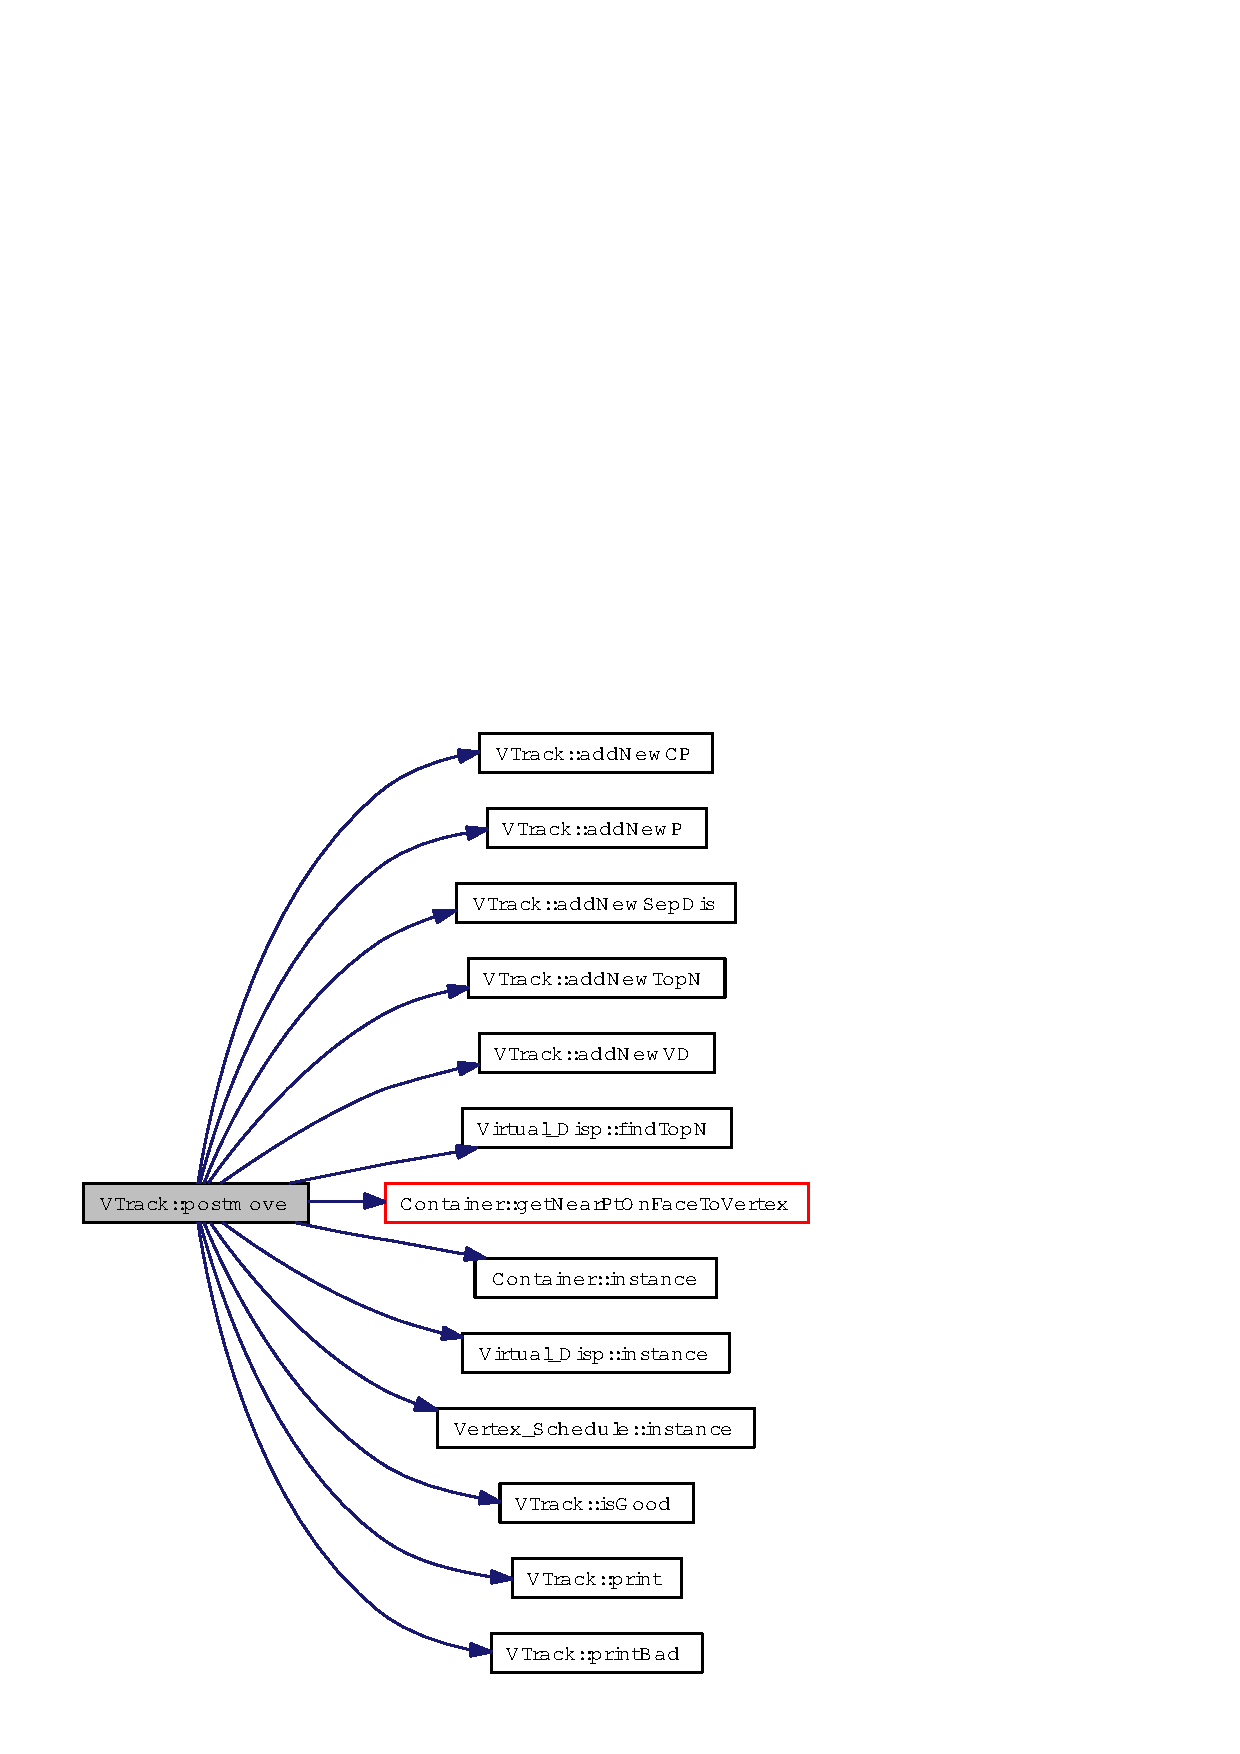
\includegraphics[width=196pt]{classVTrack_6cc3f121ae5886b77b7b40dee5ffe05d_cgraph}
\end{center}
\end{figure}
\index{VTrack@{VTrack}!getNewSepDis@{getNewSepDis}}
\index{getNewSepDis@{getNewSepDis}!VTrack@{VTrack}}
\subsubsection{\setlength{\rightskip}{0pt plus 5cm}double VTrack::get\-New\-Sep\-Dis (void)}\label{classVTrack_bcb8869fdc244de38ca59692bde74bae}




Definition at line 120 of file vtrack.cc.\index{VTrack@{VTrack}!getNewVD@{getNewVD}}
\index{getNewVD@{getNewVD}!VTrack@{VTrack}}
\subsubsection{\setlength{\rightskip}{0pt plus 5cm}double VTrack::get\-New\-VD (void)}\label{classVTrack_8771b40859350a138ba1219bdb46301a}




Definition at line 130 of file vtrack.cc.\index{VTrack@{VTrack}!getNewTopN@{getNewTopN}}
\index{getNewTopN@{getNewTopN}!VTrack@{VTrack}}
\subsubsection{\setlength{\rightskip}{0pt plus 5cm}double VTrack::get\-New\-Top\-N (void)}\label{classVTrack_205f875344d638949aa1cfb9e0fc24cf}




Definition at line 140 of file vtrack.cc.\index{VTrack@{VTrack}!getOrigSepDis@{getOrigSepDis}}
\index{getOrigSepDis@{getOrigSepDis}!VTrack@{VTrack}}
\subsubsection{\setlength{\rightskip}{0pt plus 5cm}double VTrack::get\-Orig\-Sep\-Dis (void)}\label{classVTrack_4e059529206f0a3976419db7f13a95a7}




Definition at line 150 of file vtrack.cc.\index{VTrack@{VTrack}!getOrigVD@{getOrigVD}}
\index{getOrigVD@{getOrigVD}!VTrack@{VTrack}}
\subsubsection{\setlength{\rightskip}{0pt plus 5cm}double VTrack::get\-Orig\-VD (void)}\label{classVTrack_5b3876ee487b2781cb543cb52c05c477}




Definition at line 160 of file vtrack.cc.\index{VTrack@{VTrack}!getOrigTopN@{getOrigTopN}}
\index{getOrigTopN@{getOrigTopN}!VTrack@{VTrack}}
\subsubsection{\setlength{\rightskip}{0pt plus 5cm}double VTrack::get\-Orig\-Top\-N (void)}\label{classVTrack_d178652438da940c67e6f546f73d9bfd}




Definition at line 170 of file vtrack.cc.\index{VTrack@{VTrack}!getVertex@{getVertex}}
\index{getVertex@{getVertex}!VTrack@{VTrack}}
\subsubsection{\setlength{\rightskip}{0pt plus 5cm}{\bf Vertex} $\ast$ VTrack::get\-Vertex (void)}\label{classVTrack_e2c7d468b6dbfcc1536ab13eef5c331c}




Definition at line 90 of file vtrack.cc.

The documentation for this class was generated from the following files:\begin{CompactItemize}
\item 
{\bf vtrack.h}\item 
{\bf vtrack.cc}\end{CompactItemize}
